\documentclass[12pt]{article}
\usepackage[utf8]{inputenc}
\usepackage{amsmath,amssymb}
\usepackage{float}
\usepackage{graphicx}
\usepackage[a4paper, margin=2.54cm]{geometry}
\usepackage{enumerate}
\usepackage{xcolor}
\usepackage{caption}
\usepackage{fancyhdr}
\usepackage{pgfplots}
\usepackage{enumitem}
\usepackage{tikz}
\usepackage{physics}
\usepackage{tikz-3dplot} % Permite coordenadas 3D
% Definir un comando para el número de pregunta en azul
\newcommand{\question}[1]{\textcolor{blue}{\textbf{#1}}}
%\usepackage[spanish]{babel}
\setlength{\headheight}{14.5pt} % Ajustar la altura del encabezado
\usetikzlibrary{3d}
\pagestyle{fancy}
\fancyhf{}
\fancyhead[L]{Taller No. 5-Teoría Electromagnética}
\fancyfoot[R]{ \thepage}
\renewcommand{\footrulewidth}{0.4pt}



\begin{document}
\begin{titlepage}
        \begin{center}
            \LARGE \textbf{Taller No. 3\\Teoría Electromagnética}
            \vfill
            \large

            Karen Alejandra Freire Rosero\\
            Sonier Andrés Ortiz Castelblanco\\
            Sarah Isabel Tejada García\\
            Santiago Alejandro Pérez Ramos
            \vfill
            \textbf{Asignatura:} Teoría Electromagnética\\
            \textbf{Profesor:} Servio Tulio Pérez Merchancano, Ph.D\\
            \vfill
            Universidad del Cauca\\
            Facultad de Ciencias Naturales, Exactas y de la Educación\\
            Departamento de Física\\
            Popayán, Cauca\\
            2025
        \end{center}
\end{titlepage}

\section*{\question{Problema 3.13}}

Encuentra el potencial en la ranura infinita del Ejercicio 3.3 si la frontera en \(x=0\) consiste en dos tiras metálicas: una, desde \(y=0\) hasta \(y=a/2\), está a un potencial constante \( V_0\), y la otra, desde \(y=a/2\) hasta \(y=a\), está a un potencial de \( -V_0 \).

\subsection*{Solución}
Antes de realizar el problema 3.13 y 3.14, resolveremos el Ejercicio 3.3.

\subsection*{Ejercicio 3.3}
Dos placas metálicas infinitas conectadas a tierra se encuentran paralelas al plano \(xz\), una ubicada en \(y=0\), y la otra en \(y=a\) (ver Fig. 3.17). El extremo izquierdo, en \(x=0\), está cerrado con una banda infinita aislada de las dos placas, y se mantiene a un potencial específico \( V_0(y)\). Encuentra el potencial dentro de esta "ranura" (slot).

\begin{figure}[h]
    \centering
    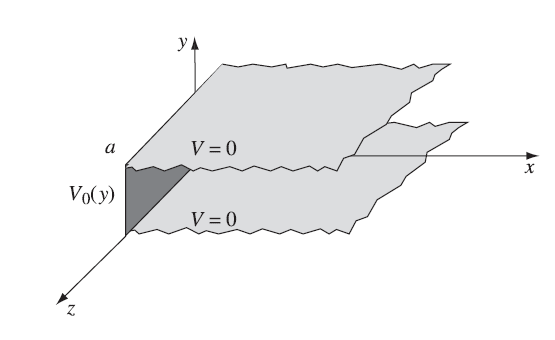
\includegraphics[width=0.75\linewidth]{imagenes/Fig 3.17.PNG}
    \caption*{Figura 3.17}
    \label{fig:enter-label}
\end{figure}

Sujeto a las condiciones de contorno:
\[
\left\{
\begin{array}{ll}
\text{(i)} & V = 0 \quad \text{cuando } y = 0, \\
\text{(ii)} & V = 0 \quad \text{cuando } y = a, \\
\text{(iii)} & V = V_0(y) \quad \text{cuando } x = 0, \\
\text{(iv)} & V \to 0 \quad \text{si } x \to \infty.
\end{array}
\right.
\]

\subsection*{Solución}

La configuración es independiente de \( z \), ya que todo es infinito en esta dirección.  
Por tanto, el problema se reduce a dos dimensiones \( (x, y) \).

\subsection*{Ecuación de Laplace}
\[
\frac{\partial^2 V}{\partial x^2} + \frac{\partial^2 V}{\partial y^2} = 0
\]

Proponemos como solución:
\[
V(x,y) = X(x)Y(y)
\]

Sustituimos en la ecuación de Laplace:
\[
Y \frac{d^2 X}{d x^2} + X \frac{d^2 Y}{d y^2} = 0
\]

Dividimos entre \( XY \):
\[
\frac{1}{X} \frac{d^2 X}{d x^2} + \frac{1}{Y} \frac{d^2 Y}{d y^2} = 0
\]

Como la primera parte depende solo de \(x\) y la segunda solo de \(y\), ambas deben ser iguales a una constante:
\[
\frac{1}{X} \frac{d^2 X}{d x^2} = C_1, \quad \frac{1}{Y} \frac{d^2 Y}{d y^2} = C_2
\]

Con:
\[
C_1 + C_2 = 0
\]

\[
C_1 = -C_2 = k^2
\]
Igualamos a \(k^2\)
\[
\frac{d^2 X}{d x^2} = k^2 X, \quad \frac{d^2 Y}{d y^2} = -k^2 Y
\]

Sean las soluciones:
\[
X(x) = A e^{k x} + B e^{-k x}
\]

\[
Y(y) = C \sin(k y) + D \cos(k y)
\]


\subsection*{Soluciones generales}

\subsection*{Para \( Y(y) \):}
\[
\frac{d^2 Y}{dy^2} = -k^2 Y, \quad Y(y) = C \sin(ky) + D \cos(ky)
\]

Aplicamos condiciones de frontera:
\[
y = 0 \quad \text{y} \quad y = a
\]

Si \( y=0 \Rightarrow Y(0) = C \sin(0) + D \cos(0) = 0 \)

\[
Y(0) = D = 0
\]
Entonces 
\[
\boxed{D = 0}
\]

Si \(y= a \Rightarrow Y(a) = C \sin(ka) + D \cos(ka) = 0 \) 

\[
Y(a) = C \sin(ka) = 0
\]

Para que esto se cumpla con \( C \ne 0 \) (queremos soluciones no triviales), necesitamos:

\[
\sin(ka) = 0 \quad \Rightarrow \quad ka = n\pi \quad ; \quad k = \frac{n\pi}{a}
\]
De forma general,
\[
\boxed{Y(y) = \sin\left(\frac{n\pi y}{a}\right), \quad \text{con } n = 1, 2, 3, \ldots}
\]

\subsection*{Para \( X(x) \):}

\[
\frac{d^2 X}{dx^2} = k^2 X \quad ; \quad X(x) = A e^{kx} + B e^{-kx}
\]

Como \( k = \frac{n\pi}{a} \), entonces:
\[
X(x) = A e^{\frac{n\pi}{a}x} + B e^{-\frac{n\pi}{a}x}
\]

Pero como \( V = 0 \) cuando \( x \to \infty \):

\[
X(x) = A e^{\infty} + B e^{-\infty} = 0
\]

Entonces \(A \) debe ser \( 0\) para que no tienda a \(\infty\)

\[
\boxed{X(x) = B e^{-\frac{n\pi}{a}x}}
\]


Finalmente, la solución general:

\[
\boxed{V(x,y) = \sum_{n=1}^{\infty} C_n e^{-\frac{n \pi}{a} x} \sin\left( \frac{n \pi}{a} y \right)} \tag{1}
\]

Determinamos los coeficientes \( C_n \) usando la condición de contorno (iii) \( V = V_0(y) \) en \( x=0 \):

\[
V(0,y) = V_0(y) = \sum_{n=1}^{\infty} C_n e^{0} \sin\left( \frac{n \pi}{a} y \right)
\]

\[
V_0(y) = \sum_{n=1}^{\infty} C_n \sin\left( \frac{n \pi}{a} y \right) \tag{*}
\]

La suma es una serie de Fourier senoidal. Multiplicamos ambos lados de la serie por \( \sin\left( \frac{n' \pi}{a} y \right) \) e integramos en \( y \) de 0 a \( a \):

\[
\int_0^a V_0(y) \sin\left( \frac{n' \pi}{a} y \right) dy = \sum_{n=1}^{\infty} C_n \int_0^a \sin\left( \frac{n \pi}{a} y \right) \sin\left( \frac{n' \pi}{a} y \right) dy
\]

Usamos ortogonalidad:

\[
\int_0^a \sin\left( \frac{n \pi}{a} y \right) \sin\left( \frac{n' \pi}{a} y \right) dy = 
\begin{cases}
0, & \text{si } n' \neq n \\
\frac{a}{2}, & \text{si } n' = n
\end{cases}
\]

Si \( n' = n \), entonces:

\[
\int_0^a V_0(y) \sin\left( \frac{n \pi}{a} y \right) dy = \frac{a}{2} \sum_{n=1}^{\infty} C_n
\]

Despejando Cn:

\[
\boxed{C_n = \frac{2}{a} \int_0^a V_0(y) \sin\left( \frac{n \pi}{a} y \right) dy} \tag{2}
\]

Si el potencial en \( x = 0 \) es una constante \( V_0 = V_0(y) \):

\[
C_n = \frac{2V_0}{a} \left[ \int_0^a \sin\left( \frac{n\pi}{a} y \right) dy \right]
\]
Resolvemos la integral, sustituimos \( u = \frac{n\pi}{a}y \), entonces:

\[
C_n = \frac{2V_0}{a} \left[ \frac{a}{n\pi} (-\cos u) \Big|_0^{n\pi} \right]
\]

\[
C_n = \frac{2V_0}{a} \left[ \frac{a}{n\pi} \left( -\cos(n\pi) + \cos(0) \right) \right]
\]

\[
C_n = \frac{2V_0}{a} \cdot \frac{a}{n\pi} \left( 1 - \cos(n\pi) \right)
\]

\[
C_n = \frac{2V_0}{n\pi} (1 - \cos(n\pi)) =
\begin{cases}
0, & \text{si } n \text{ es par} \\
\frac{4V_0}{n\pi}, & \text{si } n \text{ es impar}
\end{cases}
\]

Por lo tanto, la solución es:

\[
\boxed{V(x,y) = \sum_{\substack{n=1 \\ n \text{ impar}}}^{\infty} \frac{4V_0}{n\pi} e^{-\frac{n\pi}{a}x} \sin\left( \frac{n\pi}{a} y \right)} \tag{3}
\]

\vspace{0.7cm}

\subsection*{Solución ejercicio 3.13}

Partimos de las soluciones generales (1) y (2) del ejercicio 3.3:

\[
V(x,y) = \sum_{n=1}^{\infty} C_n e^{-\frac{n\pi}{a}x} \sin\left( \frac{n\pi}{a} y \right)
\]

donde:

\[
C_n = \frac{2}{a} \int_0^a V_0(y) \sin\left( \frac{n\pi}{a} y \right) dy
\]

Para este caso en la frontera con \( x = 0 \):

\[
V_0(y) =
\begin{cases}
V_0,  & 0 \leq y < \frac{a}{2} \\
-V_0, & \frac{a}{2} < y \leq a
\end{cases}
\]

Partimos la integral por tramos:

\[
C_n = \frac{2V_0}{a} \left[ \int_0^{a/2} \sin\left( \frac{n\pi}{a} y \right) dy - \int_{a/2}^{a} \sin\left( \frac{n\pi}{a} y \right) dy \right]
\]

Sabemos que:

\[
\int \sin(ky) \, dy = -\frac{1}{k} \cos(ky), \quad \text{con } k = \frac{n\pi}{a}
\]

Evaluamos:\\

\textbf{Primer término:}

\[
\int_0^{a/2} \sin\left( \frac{n\pi}{a} y \right) dy = -\frac{a}{n\pi} \left[ \cos\left( \frac{n\pi}{a} y \right) \right]_0^{a/2}
= -\frac{a}{n\pi} \left[ \cos\left( \frac{n\pi}{2} \right) - 1 \right]
\]

\textbf{Segundo término:}

\[
\int_{a/2}^{a} \sin\left( \frac{n\pi}{a} y \right) dy = -\frac{a}{n\pi} \left[ \cos\left( \frac{n\pi}{a} y \right) \right]_{a/2}^{a}
= -\frac{a}{n\pi} \left[ \cos(n\pi) - \cos\left( \frac{n\pi}{2} \right) \right]
\]

Tenemos,
\[
C_n = \frac{2V_0}{a} \left[ -\frac{a}{n\pi} (\cos\left( \frac{n\pi}{2} \right) - 1) + \frac{a}{n\pi} (\cos(n\pi) - \cos\left( \frac{n\pi}{2} \right)) \right]
\]

\[
C_n = \frac{2V_0}{n\pi} \left[ -\cos\left( \frac{n\pi}{2} \right) + 1 + \cos(n\pi) - \cos\left( \frac{n\pi}{2} \right) \right]
\]

\[
C_n = \frac{2V_0}{n\pi} \left[ -2\cos\left( \frac{n\pi}{2} \right) + 1 + \cos(n\pi) \right]
\]

Ahora analizamos:\\

\textbf{Para \( n \) par:}

\[
\cos(n\pi) = 1, \quad \cos\left( \frac{n\pi}{2} \right) = \pm 1
\]

\[
n = 2 \Rightarrow C_2 = \frac{2V_0}{2\pi} \left[ -2(-1) + 1 + 1 \right] = \frac{2V_0}{2\pi}(4) = \frac{4V_0}{\pi}
\]

\[
n = 4 \Rightarrow C_4 = \frac{2V_0}{4\pi} \left[ -2(1) + 1 + 1 \right] = 0 \Rightarrow C_4 = 0
\]

\textbf{Para \( n \) impar:}

\[
\cos(n\pi) = -1, \quad \cos\left( \frac{n\pi}{2} \right) = 0
\]

\[
n = 1 \Rightarrow C_1 = \frac{2V_0}{\pi} (-2(0) + 1 - 1) = 0
\]

\[
n = 3 \Rightarrow C_3 = \frac{2V_0}{3\pi} (-2(0) + 1 - 1) = 0
\]

Luego:
\[
C_n =
\begin{cases}
\frac{8V_0}{n\pi}, & \text{si } n = 2, 6, 10, 14 \quad \text{(para } n = 4j + 2, \ j = 0, 1, 2, \dots) \\
0, & \text{de otra manera}
\end{cases}
\]

Finalmente,
\[
\boxed{V(x,y) = \frac{8V_0}{\pi} \sum_{n=2,6,10,\dots}^{\infty} \frac{1}{n} e^{-\frac{n\pi}{a}x} \sin\left( \frac{n\pi}{a}y \right)}
\]

o también,
\[
\boxed{V(x,y) = \frac{8V_0}{\pi} \sum_{j=0}^{\infty} \frac{e^{-\frac{(4j+2)\pi}{a}x} \sin\left( \frac{(4j+2)\pi}{a}y\right)}{(4j+2)}  }
\]\\


\section*{\textcolor{blue}{Problema 3.14}}

Para la ranura infinita  (Ejercicio 3.3), determina la densidad de carga \( \sigma(y) \) sobre la tira en \( x = 0 \), asumiendo que es un conductor a potencial constante \( V_0 \).

\subsection*{Solución}

Partimos de la Ec. 3, solución del Ejercicio. 3.3:
\[
V(x,y) = \frac{4V_0}{\pi} \sum_{n=1,3,5}^{\infty} \frac{1}{n} e^{-\frac{n\pi}{a}x} \sin\left( \frac{n\pi}{a}y \right)
\]

La ecuación 2.49 del libro:

\[
\sigma = -\varepsilon_0 \frac{\partial V}{\partial n}
\]

donde \( \frac{\partial}{\partial n} \) es la derivada normal hacia afuera del conductor. En este caso el conductor está en \( x = 0 \), entonces:

\[
\sigma(y) = -\varepsilon_0 \left. \frac{\partial V}{\partial x} \right|_{x=0}
\]

Reemplazamos,

\[
\sigma(y) = -\varepsilon_0 \frac{\partial}{\partial x} \left[ \frac{4V_0}{\pi} \sum_{n=1,3,5}^\infty \frac{1}{n} e^{-\frac{n\pi}{a}x} \sin\left( \frac{n\pi}{a} y \right) \right]
\]

\[
= -\varepsilon_0 \cdot \frac{4V_0}{\pi} \sum_{n=1,3,5}^\infty \frac{1}{n} \sin\left( \frac{n\pi}{a} y \right) \frac{\partial}{\partial x} \left( e^{-\frac{n\pi}{a}x} \right)
\]

\[
= -\varepsilon_0 \cdot \frac{4V_0}{\pi} \sum_{n=1,3,5}^\infty \frac{1}{n} \sin\left( \frac{n\pi}{a} y \right) \left( -\frac{n\pi}{a} \right) e^{-\frac{n\pi}{a}x} \bigg|_{x=0}
\]

\[
= -\varepsilon_0 \cdot \frac{4V_0}{\pi} \left( -\frac{\pi}{a} \right) \sum_{n=1,3,5}^\infty \sin\left( \frac{n\pi}{a} y \right)
\]

Obtenemos finalmente,
\[
\boxed{
\sigma(y) = \frac{4V_0 \varepsilon_0}{a} \sum_{n=1,3,5}^\infty \sin\left( \frac{n\pi}{a} y \right)
}
\]

 \section*{\question{Problema 3.17:}} Derivar el polinomio de Legendre \( P_3(x) \) utilizando la fórmula de Rodrigues. Y demuestre  que \( P_3(\cos\theta) \) satisface la ecuación angular (3.60)  para \( l = 3 \).
  Demuestre que \( P_3(x) \) y \( P_1(x) \) son ortogonales  mediante integración explícita.

\section*{1. Derivación de \( P_3(x) \) con la fórmula de Rodrigues}

La fórmula de Rodrigues para los polinomios de Legendre está dada por:

\[
P_l(x) = \frac{1}{2^l l!} \frac{d^l}{dx^l} \left( x^2 - 1 \right)^l
\]

Para el caso \( l = 3 \), se tiene:

\[
P_3(x) = \frac{1}{8 \cdot 6} \frac{d^3}{dx^3} \left( x^2 - 1 \right)^3
\]

Calculando el polinomio:

\[
(x^2 - 1)^3 = x^6 - 3x^4 + 3x^2 - 1
\]

Derivando tres veces:

\begin{align*}
\frac{d}{dx} &= 6x^5 - 12x^3 + 6x \\
\frac{d^2}{dx^2} &= 30x^4 - 36x^2 + 6 \\
\frac{d^3}{dx^3} &= 120x^3 - 72x
\end{align*}

Entonces:

\[
P_3(x) = \frac{1}{48} (120x^3 - 72x) = \frac{5}{2}x^3 - \frac{3}{2}x
\]

\[
\boxed{P_3(x) = \frac{5}{2}x^3 - \frac{3}{2}x}
\]

\subsection*{2. Verificación de la ecuación angular}

La ecuación angular de Legendre está dada por:

\[
\frac{1}{\sin\theta} \frac{d}{d\theta} \left( \sin\theta \frac{d\Theta}{d\theta} \right) + l(l+1)\Theta = 0,
\]

para \( l = 3 \) y \( \Theta(\theta) = P_3(\cos\theta) \).

Se tiene que:

\[
\Theta(\theta) = P_3(\cos\theta) = \frac{5}{2} \cos^3\theta - \frac{3}{2} \cos\theta.
\]

Calculando su derivada con respecto a \( \theta \):

\begin{align*}
\frac{d\Theta}{d\theta} &= \frac{d}{d\theta} \left( \frac{5}{2} \cos^3\theta - \frac{3}{2} \cos\theta \right) \\
&= \frac{5}{2} \cdot 3 \cos^2\theta (-\sin\theta) + \frac{3}{2} \sin\theta \\
&= -\frac{15}{2} \cos^2\theta \sin\theta + \frac{3}{2} \sin\theta \\
&= \sin\theta \left( -\frac{15}{2} \cos^2\theta + \frac{3}{2} \right)
\end{align*}

Multiplicando por \( \sin\theta \):

\[
\sin\theta \frac{d\Theta}{d\theta} = \sin^2\theta \left( -\frac{15}{2} \cos^2\theta + \frac{3}{2} \right)
\]

Luego, derivando de nuevo:

\begin{align*}
\frac{d}{d\theta} \left( \sin\theta \frac{d\Theta}{d\theta} \right) &= \frac{d}{d\theta} \left[ \sin^2\theta \left( -\frac{15}{2} \cos^2\theta + \frac{3}{2} \right) \right] \\
&= \frac{d}{d\theta} \left[ -\frac{15}{2} \sin^2\theta \cos^2\theta + \frac{3}{2} \sin^2\theta \right]
\end{align*}

Usando identidades trigonométricas:

\[
\sin^2\theta = \frac{1 - \cos(2\theta)}{2}, \quad \cos^2\theta = \frac{1 + \cos(2\theta)}{2}
\]

Al simplificar, se obtiene finalmente:

\[
\frac{1}{\sin\theta} \frac{d}{d\theta} \left( \sin\theta \frac{d\Theta}{d\theta} \right) = -12 \Theta(\theta),
\]

ya que \( l = 3 \Rightarrow l(l+1) = 12 \), lo cual verifica que \( \Theta(\theta) = P_3(\cos\theta) \) satisface la ecuación angular.

\[
\boxed{\text{Por tanto, } \Theta(\theta) = P_3(\cos\theta) \text{ satisface la ecuación angular para } l = 3.}
\]

\subsection*{3. Verificación de la ortogonalidad entre \( P_3(x) \) y \( P_1(x) \)}

Se verifica la ortogonalidad utilizando la propiedad:

\[
\int_{-1}^1 P_l(x) P_{l'}(x) dx = 0 \quad \text{si } l \ne l'
\]

Se tiene:

\[
P_1(x) = x, \quad P_3(x) = \frac{5}{2}x^3 - \frac{3}{2}x
\]

Producto:

\[
P_1(x) P_3(x) = x\left( \frac{5}{2}x^3 - \frac{3}{2}x \right) = \frac{5}{2}x^4 - \frac{3}{2}x^2
\]

Integramos:

\begin{align*}
\int_{-1}^1 \left( \frac{5}{2}x^4 - \frac{3}{2}x^2 \right) dx &= \frac{5}{2} \int_{-1}^1 x^4 dx - \frac{3}{2} \int_{-1}^1 x^2 dx \\
&= \frac{5}{2} \cdot \frac{2}{5} - \frac{3}{2} \cdot \frac{2}{3} \\
&= 1 - 1 = 0
\end{align*}

\[
\boxed{\int_{-1}^1 P_1(x)P_3(x)dx = 0}
\]

Por tanto, \( P_1(x) \) y \( P_3(x) \) son ortogonales.
\vspace{5mm}
\\

\section*{\question{Problema 3.18:}}  (a)Supón que el potencial es una constante \( V_0 \) sobre la superficie de una esfera. Usa los resultados de los Ejemplos 3.6 y 3.7 para encontrar el potencial dentro y fuera de la esfera.
(b) Encuentra el potencial dentro y fuera de una cáscara esférica que lleva una densidad de carga superficial uniforme \( \sigma_0 \), usando los resultados del Ejemplo 3.9.

\subsection*{(a) Potencial constante sobre la superficie de una esfera}

Se sabe que el potencial general para problemas con simetría esférica (Ej. 3.6 y 3.7) es:

\[
V(r, \theta) = \sum_{\ell=0}^{\infty} \left( A_\ell r^\ell + \frac{B_\ell}{r^{\ell+1}} \right) P_\ell(\cos\theta)
\]

Para el interior de la esfera ($r < R$), se tiene que  $B_\ell = 0$, por lo que:

\[
V_{\text{dentro}}(r, \theta) = \sum_{\ell=0}^{\infty} A_\ell r^\ell P_\ell(\cos\theta)
\]

Para el exterior de la esfera ($r > R$), $A_\ell = 0$, y se tiene:

\[
V_{\text{fuera}}(r, \theta) = \sum_{\ell=0}^{\infty} \frac{B_\ell}{r^{\ell+1}} P_\ell(\cos\theta)
\]

Como la condición de frontera es que $V(R, \theta) = V_0$, y $V_0$ es constante, esto implica que solo sobrevive el término $\ell = 0$:
Por dentro: 
\[
V_0 = A_0 R^0 P_0(\cos\theta) = A_0
\]
\[
V_{\text{dentro}}(r, \theta) = V_0
\]
Por fuera:
\[
V_0 = \frac{B_0}{R} P_0(\cos\theta) = \frac{B_0}{R}
\]

\[
B_0= \frac{V_0}{R}
\]
\[
V_{\text{fuera}}(r, \theta) = \frac{V_0 R}{r}
\]

Entonces, el potencial total es:

\[
V(r, \theta) =
\begin{cases}
V_0, & r < R \\
\displaystyle \frac{V_0 R}{r}, & r > R
\end{cases}
\]
\subsection*{(b) Cáscara esférica con densidad superficial uniforme \( \sigma_0 \)}

Del ejemplo 3.9 se tiene:
\[
\varepsilon_0 \sum_{\ell=0}^{\infty} (2\ell + 1) A_\ell R^{\ell - 1} P_\ell(\cos\theta) = \sigma_0
\]

Como $\sigma_0$ es constante, sólo sobrevive el término con $\ell = 0$ (polinomio de Legendre $P_0(\cos\theta) = 1$). Entonces:

\[
\varepsilon_0 \cdot A_0 \cdot \frac{1}{R} = \sigma_0
\Rightarrow
A_0 = \frac{\sigma_0 R}{\varepsilon_0}
\]

Y 
\[
B_0 = \frac{\sigma_0 R^2}{\varepsilon_0}
\]

Así que el potencial en todo el espacio es:

\[
V(r) = 
\begin{cases}
\displaystyle \frac{R \sigma_0}{\varepsilon_0}, & r < R \\
\displaystyle \frac{R^2 \sigma_0}{\varepsilon_0 r}, & r > R
\end{cases}
\]

\section*{\question{Problema 3.22}}
En el Problema 2.25, encontraste el potencial sobre el eje de un disco uniformemente cargado: 
\[ V(r,\theta) = \frac{\sigma}{2\epsilon_o}(\sqrt{r^2 + R^2}-r)\]
\begin{enumerate}[label=(\alph*)]
  \item   Usa esto, junto con el hecho de que \(P_l(1) = 1\) para evaluar los tres primeros términos en la expansión (Ecuación 3.72) para el potencial del disco en puntos fuera del eje, suponiendo que \(r > R\).

  \item  Encuentra el potencial para \(r < R\) usando el mismo método, empleando la Ecuación 3.66. [Nota: dividir la región interior en dos hemisferios, por arriba y por debajo del disco. No asumir que los coeficientes \(A_l\) son los mismos en ambos hemisferios.]
\end{enumerate}

\subsection*{Solución}
En el Problema 2.25, el potencial sobre el eje de un disco uniformemente cargado de radio \(R\):
\[
V(r,0) \;=\; \frac{\sigma}{2\varepsilon_{0}}\bigl(\sqrt{r^{2} + R^{2}} - r \bigr).
\]


\subsection*{(a) Expansión para \(\boldsymbol{r>R}\)}

Para puntos fuera del disco (\(r>R\)),  el potencial puede expresarse de la forma:
\[
V(r,\theta)
\;=\;
\sum_{l=0}^{\infty} B_{l}\,\frac{P_{l}(\cos\theta)}{r^{\,l+1}}.
\]
En particular, en el eje \(\theta=0\), como \(P_{l}(1)=1\), se tiene
\[
V(r,0)
\;=\;
\sum_{l=0}^{\infty} \frac{B_{l}}{r^{\,l+1}}.
\]

Por otro lado, para \(r>R\) la expresión dada en el enunciado es

\[
V(r,0) \;=\; \frac{\sigma}{2\varepsilon_{0}} \Bigl(\sqrt{r^{2}+R^{2}} - r\Bigr).
\]
Expandiendo \(\sqrt{r^{2}+R^{2}} - r\) en potencias de \(R/r\) cuando \(r>R\):
\begin{align*}
\sqrt{r^{2}+R^{2}} 
&= r\,\sqrt{1 + \frac{R^{2}}{r^{2}}}
= r \Bigl( 1 + \tfrac{1}{2}\,\frac{R^{2}}{r^{2}} - \tfrac{1}{8}\,\frac{R^{4}}{r^{4}} 
      + \tfrac{1}{16}\,\frac{R^{6}}{r^{6}} + \cdots \Bigr), \\
%
\sqrt{r^{2}+R^{2}} - r 
&= r\Bigl(1 + \tfrac{1}{2}\frac{R^{2}}{r^{2}} - \tfrac{1}{8}\frac{R^{4}}{r^{4}} 
          + \tfrac{1}{16}\frac{R^{6}}{r^{6}} + \cdots - 1\Bigr) \\
&= \frac{R^{2}}{2r} 
   \;-\; \frac{R^{4}}{8\,r^{3}} 
   \;+\; \frac{R^{6}}{16\,r^{5}} 
   \;-\; \cdots.
\end{align*}
Por tanto,
\[
V(r,0) 
= \frac{\sigma}{2\varepsilon_{0}} 
  \left(\tfrac{R^{2}}{2r} - \tfrac{R^{4}}{8\,r^{3}} + \tfrac{R^{6}}{16\,r^{5}} - \cdots \right)
= \frac{\sigma R^{2}}{4\varepsilon_{0}}\,\frac{1}{r} 
  \;-\; \frac{\sigma R^{4}}{16\varepsilon_{0}}\,\frac{1}{r^{3}} 
  \;+\; \frac{\sigma R^{6}}{32\varepsilon_{0}}\,\frac{1}{r^{5}} 
  \;-\; \cdots.
\]
Comparando este desarrollo con
\(\displaystyle
V(r,0)=\sum_{l=0}^{\infty} \frac{B_{l}}{r^{\,l+1}},
\)
Tenemos que los tres primeros coeficientes no nulos \(B_{l}\) son:
\[
\begin{aligned}
B_{0} &= \frac{\sigma\,R^{2}}{4\,\varepsilon_{0}}, \\[6pt]
B_{2} &= -\,\frac{\sigma\,R^{4}}{16\,\varepsilon_{0}}, \\[6pt]
B_{4} &= \frac{\sigma\,R^{6}}{32\,\varepsilon_{0}}\,.
\end{aligned}
\]

Así, la aproximación con los tres primeros términos para \(r>R\) queda:
\[
V(r,\theta)
\approx
\frac{\sigma\,R^{2}}{4\,\varepsilon_{0}}\,\frac{P_{0}(\cos\theta)}{r}
\;-\;
\frac{\sigma\,R^{4}}{16\,\varepsilon_{0}}\,\frac{P_{2}(\cos\theta)}{r^{3}}
\;+\;
\frac{\sigma\,R^{6}}{32\,\varepsilon_{0}}\,\frac{P_{4}(\cos\theta)}{r^{5}}.
\]

\[
V(r,\theta)\approx
\frac{\sigma\,R^{2}}{4\,\varepsilon_{0}}\;\frac{1}{r}
\;-\;
\frac{\sigma\,R^{4}}{16\,\varepsilon_{0}}\;\frac{\displaystyle \frac{1}{2}\bigl(3\cos^{2}\theta - 1\bigr)}{r^{3}}
\;+\;
\frac{\sigma\,R^{6}}{32\,\varepsilon_{0}}\;\frac{\displaystyle \frac{1}{8}\bigl(35\cos^{4}\theta - 30\cos^{2}\theta + 3\bigr)}{r^{5}}\,.
\]

\[
V(r,\theta)\approx
\frac{\sigma\,R^{2}}{4\,\varepsilon_{0}\,r} \left( 
1 \;-\;
\frac{R^{2}}{4}\,\frac{\displaystyle \frac{1}{2}\bigl(3\cos^{2}\theta - 1\bigr)}{r^{2}}
\;+\;
\frac{R^{4}}{8\,}\;\frac{\displaystyle \frac{1}{8}\bigl(35\cos^{4}\theta - 30\cos^{2}\theta + 3\bigr)}{r^{4}}\,.
\right)\]
\bigskip

\subsection*{(b) Expansión para \(\boldsymbol{r<R}\)}

Para puntos dentro del disco (\(r<R\))  el potencial puede expresarse de la forma:
\[
V(r,\theta)
\;=\;
\sum_{l=0}^{\infty} A_{l}\,r^{\,l}\,P_{l}(\cos\theta).
\]
De nuevo, en el eje \(\theta=0\) se tiene \(P_{l}(1) = 1\), luego
\[
V(r,0) \;=\; \sum_{l=0}^{\infty} A_{l}\,r^{\,l}.
\]
Pero sabemos también que el valor en el eje (\(\theta=0\)) para \(r<R\) sigue siendo
\[
V(r,0) 
= \frac{\sigma}{2\varepsilon_{0}}\,\bigl(\sqrt{r^{2}+R^{2}} - r\bigr).
\]
Ahora, desarrollando \(\sqrt{r^{2}+R^{2}} - r\) en potencias de \(r/R\) cuando \(r<R\):
\begin{align*}
\sqrt{r^{2} + R^{2}}
&= R\,\sqrt{1 + \frac{r^{2}}{R^{2}}}
= R \Bigl( 1 + \frac{1}{2}\,\frac{r^{2}}{R^{2}} - \frac{1}{8}\,\frac{r^{4}}{R^{4}} 
      + \frac{1}{16}\,\frac{r^{6}}{R^{6}} + \cdots \Bigr),\\
%
\sqrt{r^{2} + R^{2}} - r
&= R - r + \frac{r^{2}}{2\,R} - \frac{r^{4}}{8\,R^{3}} + \cdots.
\end{align*}
Por tanto,
\[
V(r,0)
= \frac{\sigma}{2\varepsilon_{0}} 
  \Bigl(R - r + \tfrac{r^{2}}{2R} - \tfrac{r^{4}}{8R^{3}} + \cdots \Bigr).
\]
Agrupando por potencias de \(r\):
\[
V(r,0)
= \underbrace{\frac{\sigma\,R}{2\varepsilon_{0}}}_{A_{0}} 
  \;-\; \underbrace{\frac{\sigma}{2\varepsilon_{0}}}_{A_{1}}\,r 
  \;+\; \underbrace{\frac{\sigma}{4\,\varepsilon_{0}\,R}}_{A_{2}}\,r^{2} 
  \;+\; \cdots.
\]
De aquí leemos los primeros coeficientes \(A_{l}\):
\[
\begin{aligned}
A_{0} &= \frac{\sigma\,R}{2\,\varepsilon_{0}}, \\[6pt]
A_{1} &= -\frac{\sigma}{2\,\varepsilon_{0}}, \\[6pt]
A_{2} &= \frac{\sigma}{4\,\varepsilon_{0}\,R}, \\[6pt]
&\;\;\vdots
\end{aligned}
\]
Por lo tanto, la aproximación con los primeros términos (hasta \(r^{2}P_{2}\)) para \(r<R\) para el hemisferio norte \(V(r,\theta)\), donde \(0 \le\theta\le\pi/2\)  es:
\[
V(r,\theta)
\approx
\frac{\sigma\,R}{2\,\varepsilon_{0}}\,P_{0}(\cos\theta)
\;-\; \frac{\sigma}{2\,\varepsilon_{0}}\,r\,P_{1}(\cos\theta)
\;+\; \frac{\sigma}{4\,\varepsilon_{0}\,R}\,r^{2}\,P_{2}(\cos\theta)
\]
\[
V(r,\theta)\approx
\frac{\sigma\,R}{2\,\varepsilon_{0}}
\;-\;
\frac{\sigma\,r\,\cos\theta}{2\,\varepsilon_{0}}
\;+\;
\frac{\sigma\,r^{2}}{8\,\varepsilon_{0}\,R}\,\bigl(3\cos^{2}\theta - 1\bigr)\,.
\]

\[
V(r,\theta)\approx
\frac{\sigma\,R}{2\,\varepsilon_{0}}\left (1
\;-\;
\frac{r\,\cos\theta}{R}
\;+\;
\frac{r^{2}}{4\,R^2}\,\bigl(3\cos^{2}\theta - 1\bigr)\,\right).
\]
Ahora, para el hemisferio sur (\(\theta=\pi\)), tenemos en cuenta que \(P_{l}(-1) = (-1)^{l}\), por lo que los coeficientes \(A_{l}\) son los mismos, pero con signo alternante: 
\[ V(r,\pi) = \sum_{l=0}^{\infty} (-1)^l A_l'r^l = \frac{\sigma}{2 \epsilon_o} \left( \sqrt{r^2 + R^2} -r\right)\]

Donde los coeficientes \(A_l'\) son:
\[
\begin{aligned}
A_{0}' &= \frac{\sigma\,R}{2\,\varepsilon_{0}}, \\[6pt]
A_{1}' &= \frac{\sigma}{2\,\varepsilon_{0}}, \\[6pt]
A_{2}' &= \frac{\sigma}{4\,\varepsilon_{0}\,R}, \\[6pt]
&\;\;\vdots
\end{aligned}
\]
Por lo tanto la aproximación con los primeros términos (hasta \(r^{2}P_{2}\)) para \(r<R\) para el hemisferio sur es:
\[
V(r,\theta) \approx \frac{\sigma\,R}{2\,\varepsilon_{0}} P_{0}(\cos\theta) + \frac{\sigma}{2\,\varepsilon_{0}} r P_{1}(\cos\theta) + \frac{\sigma}{4\,\varepsilon_{0}\,R} r^{2} P_{2}(\cos\theta)\]
\[
V(r,\theta)\approx
\frac{\sigma\,R}{2\,\varepsilon_{0}}\left (1
\;+\;
\frac{r\,\cos\theta}{R}
\;+\;
\frac{r^{2}}{4\,R^2}\,\bigl(3\cos^{2}\theta - 1\bigr)\,\right).
\]
\section*{\question{Problema 3.24}}
Resuelve la ecuación de Laplace mediante separación de variables en coordenadas cilíndricas, asumiendo que no hay dependencia con respecto a z (simetría cilíndrica).

\subsection*{Solución}

La ecuación de Laplace en coordenadas cilíndricas $(\rho, \varphi, z)$, asumiendo que no hay dependencia con respecto a $z$ (simetría axial), se reduce a:

$$ \nabla^2 \Phi = \frac{1}{\rho} \frac{\partial}{\partial \rho} \left( \rho \frac{\partial \Phi}{\partial \rho} \right) + \frac{1}{\rho^2} \frac{\partial^2 \Phi}{\partial \varphi^2} = 0 $$

Proponemos una solución mediante separación de variables, de la forma $\Phi(\rho, \varphi) = S(\rho) F(\varphi)$. Sustituyendo esta forma en la ecuación de Laplace:

$$ \frac{F(\varphi)}{\rho} \frac{d}{d \rho} \left( \rho \frac{d S}{d \rho} \right) + \frac{S(\rho)}{\rho^2} \frac{d^2 F}{d \varphi^2} = 0 $$

Multiplicamos por $\frac{\rho^2}{S(\rho)F(\varphi)}$ para separar las variables:

$$ \frac{\rho}{S(\rho)} \frac{d}{d \rho} \left( \rho \frac{d S}{d \rho} \right) + \frac{1}{F(\varphi)} \frac{d^2 F}{d \varphi^2} = 0 $$

Esto nos lleva a dos ecuaciones diferenciales ordinarias, igualando cada parte a una constante de separación $k^2$
$$ \frac{\rho}{S(\rho)} \frac{d}{d \rho} \left( \rho \frac{d S}{d \rho} \right) = k^2 $$
$$ \frac{1}{F(\varphi)} \frac{d^2 F}{d \varphi^2} = -k^2 $$

\subsection*{i) Ecuación angular}
$$ \frac{d^2 F}{d \varphi^2} + k^2 F(\varphi) = 0 $$
La solución general para esta ecuación es:
$$ F(\varphi) = A_k \cos(k\varphi) + B_k \sin(k\varphi) $$

\subsection*{ii) Ecuación radial}
$$ \frac{\rho}{S(\rho)} \frac{d}{d \rho} \left( \rho \frac{d S}{d \rho} \right) = k^2 $$
$$ \rho \frac{d}{d \rho} \left( \rho \frac{d S}{d \rho} \right) - k^2 S(\rho) = 0 $$
Expandiendo el término de la derivada:
$$ \rho \left( \frac{dS}{d\rho} + \rho \frac{d^2S}{d\rho^2} \right) - k^2 S = 0 $$
$$ \rho^2 \frac{d^2S}{d\rho^2} + \rho \frac{dS}{d\rho} - k^2 S = 0 $$
Esta es la ecuación de Euler-Cauchy.

\subsection*{Caso 1: $k \neq 0$}
La solucion es de la forma $S(\rho) = \rho^m$. 
$$ \rho^2 m(m-1)\rho^{m-2} + \rho m\rho^{m-1} - k^2 \rho^m = 0 $$
$$ m(m-1) + m - k^2 = 0 $$
$$ m^2 - m + m - k^2 = 0 $$
$$ m^2 = k^2 \implies m = \pm k $$
Por lo tanto, la solución general para $S(\rho)$ cuando $k \neq 0$ (y $k$ es un entero $n \neq 0$) es:
$$ S_n(\rho) = C_n \rho^k + D_n \rho^{-k} $$

\subsection*{Caso 2: $k = 0$}
La ecuación radial se simplifica a:
$$ \rho \frac{d}{d \rho} \left( \rho \frac{d S}{d \rho} \right) = 0 $$
Dividiendo por $\rho$ (asumiendo $\rho \neq 0$):
$$ \frac{d}{d \rho} \left( \rho \frac{d S}{d \rho} \right) = 0 $$
Integrando una vez:
$$ \rho \frac{d S}{d \rho} = C_1 $$
$$ \frac{d S}{d \rho} = \frac{C_1}{\rho} $$
Integrando de nuevo:
$$ S_0(\rho) = C_1 \ln(\rho) + C_2 $$
Esta solución logarítmica es la que corresponde al potencial de una línea de carga infinita.

\section*{Solución General}

La solución general $\Phi(\rho, \varphi)$ es la superposición de todas las soluciones. 
$$ V(\rho, \varphi) = a_0 + b_0 \ln(\rho) + \sum_{k=1}^{\infty} \left[ (a_k \rho^k + b_k \rho^{-k})\cos(k\varphi) + (c_k \rho^k + d_k \rho^{-k})\sin(k\varphi) \right] $$

\section*{\question{Problema 3.25}}
Encuentra el potencial fuera de un tubo metálico infinitamente largo, de radio \( R \), colocado perpendicularmente a un campo eléctrico uniforme \( \vec{E}_0 \). Luego, encuentra la densidad de carga superficial inducida en el tubo. Usa el resultado del problema 3.24.

\begin{figure}[ht]
    \centering
    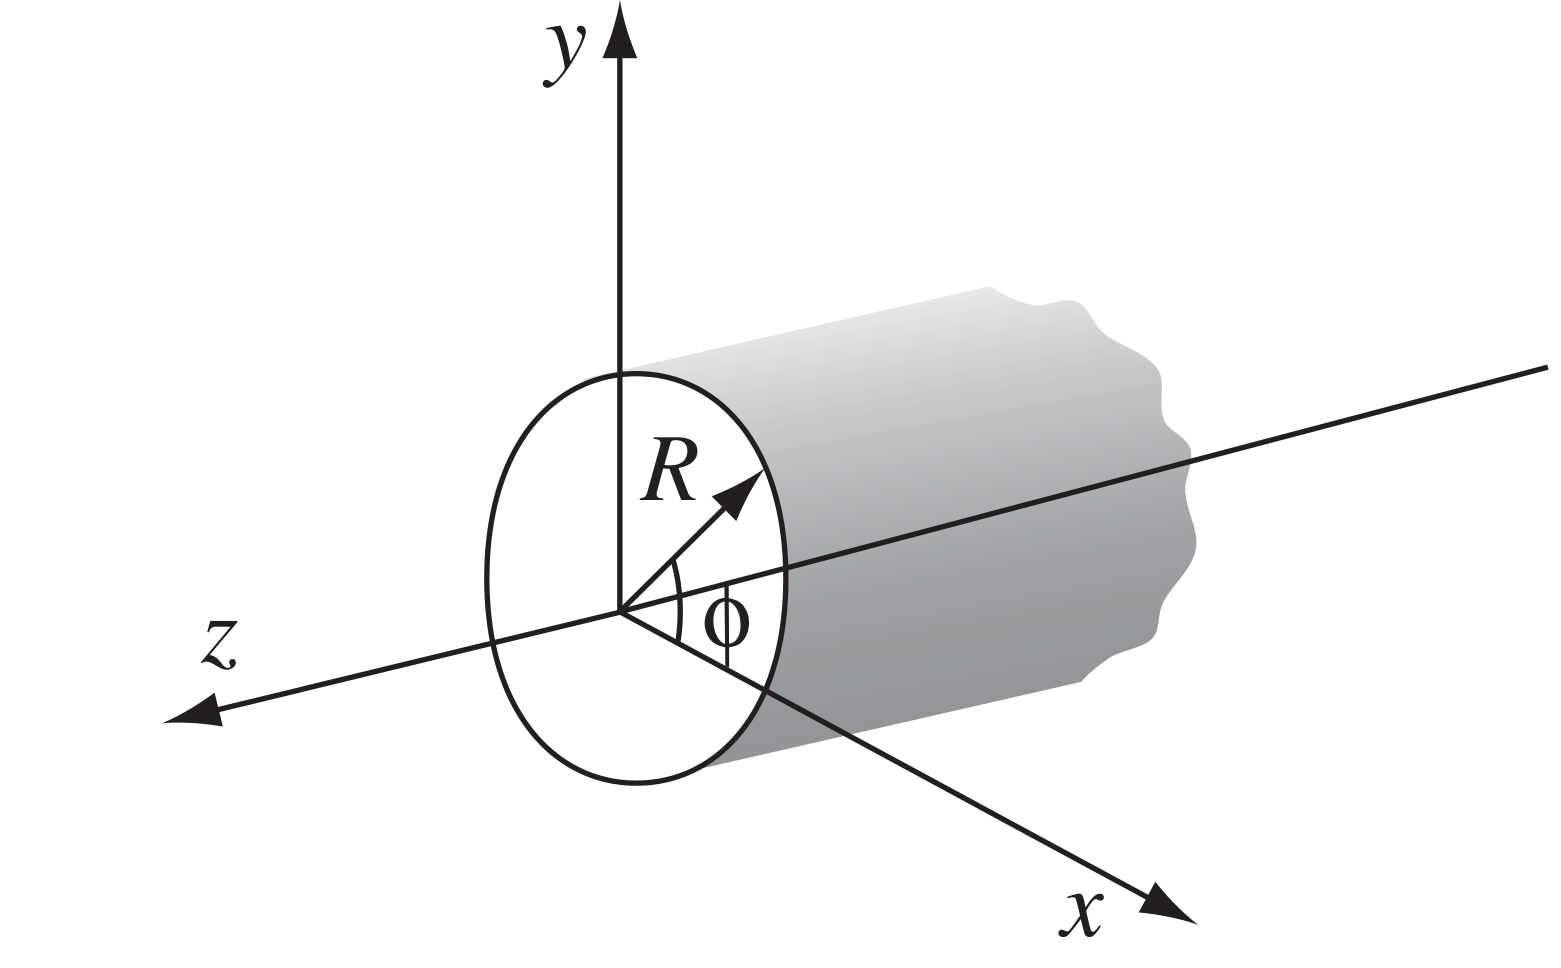
\includegraphics[width=0.5\textwidth]{imagenes/figura3.25.png}
    \caption*{Tubo metálico infinitamente cargado.}
    \label{fig:etiqueta}
\end{figure}

\textbf{Solución}

El tubo es un cilindro conductor de radio \( R \), con simetría cilíndrica (eje \( z \)). El campo eléctrico uniforme aplicado es:

\[
\vec{E}_0 = E_0 \hat{x}
\]

En coordenadas polares \( (r, \phi) \), se tiene:

\[
\vec{E}_0 = E_0 \cos \phi \, \hat{r} - E_0 \sin \phi \, \hat{\phi}
\]

El potencial asociado al campo externo es:

\[
\Phi_{\text{ext}} = -\vec{E}_0 \cdot \vec{r} = -E_0 x = -E_0 r \cos \phi
\]

\subsection*{Solución de la ecuación de Laplace}

Fuera del cilindro (región \( r > R \)), se resuelve la ecuación de Laplace en coordenadas polares:

\[
\nabla^2 \Phi = 0
\]

La solución general con simetría en \( \phi \) es:

\[
\Phi(r, \phi) = \sum_{k=1}^{\infty} \left( A_k r^k + B_k r^{-k} \right)(C_k \cos k\phi + D_k \sin k\phi)
\]

Como el campo externo solo depende de \( \cos \phi \), consideramos solo el término con \( k = 1 \) y sin seno:

\[
\Phi(r, \phi) = \left( A r + \frac{B}{r} \right) \cos \phi
\]

\subsection*{Condiciones de frontera}

\begin{itemize}
    \item En \( r = R \), el potencial debe ser cero (condición sobre el conductor):
    \[
    \Phi(R, \phi) = 0
    \]
    
    \item Para \( r \to \infty \), el potencial debe tender al del campo externo:
    \[
    \Phi(r \to \infty, \phi) \to -E_0 r \cos \phi
    \Rightarrow A = -E_0
    \]
\end{itemize}

Usando la condición en \( r = R \):

\[
\Phi(R, \phi) = \left( -E_0 R + \frac{B}{R} \right) \cos \phi = 0
\Rightarrow B = E_0 R^2
\]

\subsection*{Potencial final}

\[
\Phi(r, \phi) = \left( -E_0 r + \frac{E_0 R^2}{r} \right) \cos \phi
\]

\subsection*{Densidad superficial de carga}

La densidad superficial de carga en un conductor se relaciona con el campo eléctrico perpendicular justo fuera del conductor:

\[
\sigma(\phi) = -\varepsilon_0 \left. \frac{\partial \Phi}{\partial r} \right|_{r = R}
\]

Calculamos la derivada:

\[
\frac{\partial \Phi}{\partial r} = \left( -E_0 - \frac{E_0 R^2}{r^2} \right) \cos \phi
\]

Evaluado en \( r = R \):

\[
\left. \frac{\partial \Phi}{\partial r} \right|_{r = R} = -2 E_0 \cos \phi
\Rightarrow
\sigma(\phi) = 2 \varepsilon_0 E_0 \cos \phi
\]


\begin{itemize}
    \item Potencial fuera del tubo:
    \[
    \Phi(r, \phi) = \left( -E_0 r + \frac{E_0 R^2}{r} \right) \cos \phi
    \]

    \item Densidad superficial de carga:
    \[
    \boxed{
    \sigma(\phi) = 2 \varepsilon_0 E_0 \cos \phi
    }
       \]
\end{itemize}

\section*{\question{Problema 3.29}}

Cuatro partículas (una de carga \( q \), una de carga \( 3q \) y dos de carga \( -2q \)) se colocan como muestra la figura, cada una a una distancia \( a \) del origen. Encuentre la fórmula aproximada simple para el potencial eléctrico, válida en puntos alejados del origen. (Exprésese la respuesta en coordenadas esféricas).

\begin{figure}[h]
    \centering
    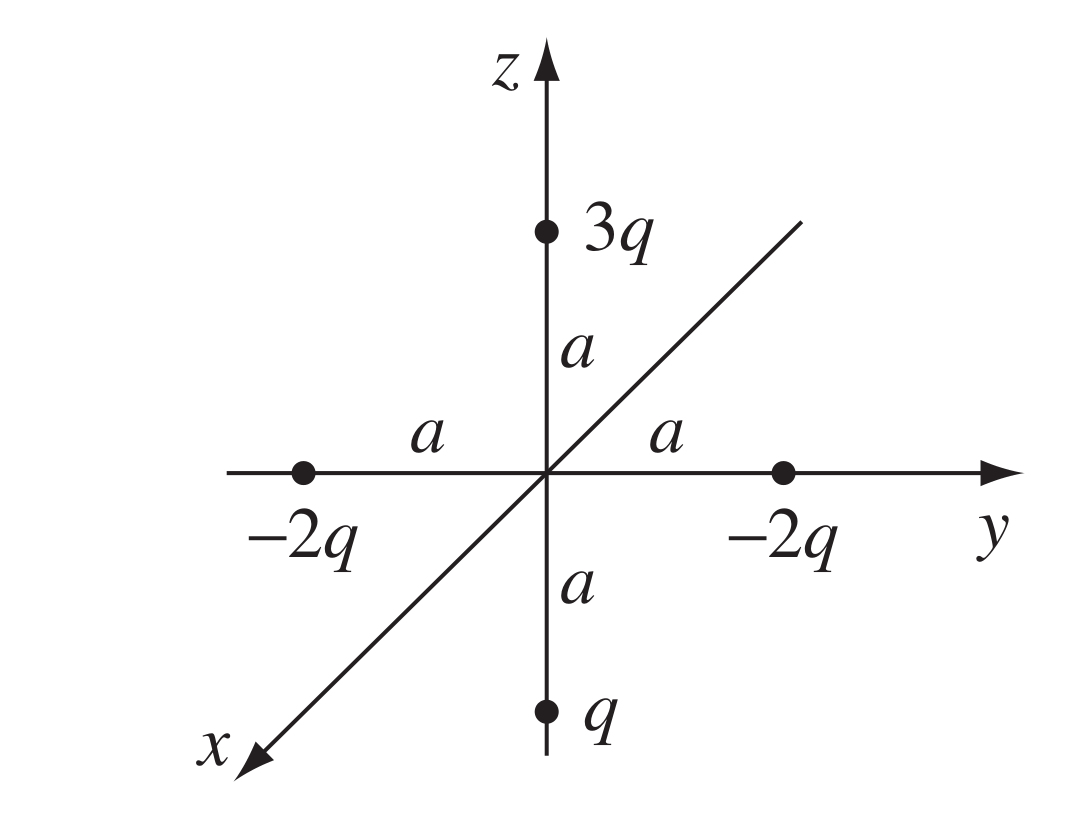
\includegraphics[width=0.5\textwidth]{imagenes/figura3.29.png}
    \caption*{Distribución de cuatro partículas con carga.}
    \label{fig:etiqueta}
\end{figure}

\subsection*{Solución}


El potencial eléctrico debido a un conjunto de cargas puntuales es:

\[
V(\vb{r}) = \frac{1}{4\pi \varepsilon_0} \sum_{i=1}^4 \frac{q_i}{\abs{\vb{r} - \vb{r}_i}}
\]

Cuando \( r \gg a \), se puede usar una expansión multipolar:

\[
V(\vb{r}) \approx \frac{1}{4\pi \varepsilon_0} \left( \frac{Q_{\text{total}}}{r} + \frac{\vb{p} \cdot \hat{\vb{r}}}{r^2} + \cdots \right)
\]

donde:
\begin{align*}
Q_{\text{total}} &= \sum_i q_i \\
\vb{p} &= \sum_i q_i \vb{r}_i
\end{align*}

\subsection*{Carga total}

\[
Q_{\text{total}} = q + 3q - 2q - 2q = 0
\]

Por lo tanto, el término monopolar se anula y el primer término no nulo es el dipolar.

\subsection*{ Momento dipolar}

Calculamos cada contribución:

\begin{align*}
q_1 \vb{r}_1 &= q (0, 0, -a) = (0, 0, -aq) \\
q_2 \vb{r}_2 &= 3q (0, 0, a) = (0, 0, 3aq) \\
q_3 \vb{r}_3 &= -2q (a, 0, 0) = (-2aq, 0, 0) \\
q_4 \vb{r}_4 &= -2q (-a, 0, 0) = (2aq, 0, 0)
\end{align*}

Sumando:

\[
\vb{p} = (-2aq + 2aq, 0, -aq + 3aq) = (0, 0, 2aq)
\]

El momento dipolar apunta en la dirección \( \hat{z} \) y tiene magnitud \( 2aq \).

\subsection*{ Potencial dipolar}

En coordenadas esféricas, el vector unitario radial es:

\[
\hat{\vb{r}} = (\sin \theta \cos \phi, \sin \theta \sin \phi, \cos \theta)
\]

Como \( \vb{p} = 2aq \hat{z} \), entonces:

\[
\vb{p} \cdot \hat{\vb{r}} = 2aq \cos \theta
\]

Finalmente, el potencial en la aproximación dipolar es:

\[
\boxed{
V(r, \theta) \approx \frac{1}{4\pi \varepsilon_0} \frac{2aq \cos \theta}{r^2}
}
\]

Este resultado muestra un comportamiento de dipolo orientado a lo largo del eje \( z \).


\end{document}